\section{Square-Wave Generator}

\subsection{Experiment Design}
    \subsubsection{Background}
        One important application of Op.Amp is that it can be used to construct signal generators. In this experiment, we will use an Op.Amp to construct a square-wave generator. And the output signal will have adjustable frequency and duty cycle.\par

    \subsubsection{Propose}
    \begin{itemize}
        \item To verify the square-wave generator
    \end{itemize}

\subsection{Experiment Design}
    \subsubsection{Materials}
        In this experiment, we will use the following components:
        \begin{itemize}
            \item 1N4148 Diode
            \item LM741 Op.Amp.
            \item Resistors
            \item Breadboard
            \item DC power supply
            \item Digital Multi-Meter
            \item Function Generator
            \item Oscilloscope
        \end{itemize}

    \subsubsection{Circuit Diagram}
        The following circuit diagrams 
        \begin{figure}[H]
            \centering
                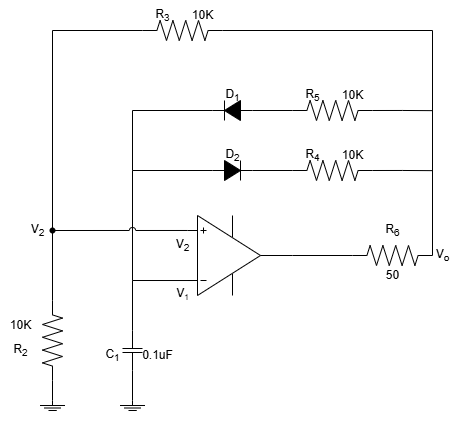
\includegraphics[width=0.6\linewidth]{Experiment_15/Circuit/Lab15.drawio.png}
                \caption{Square-Wave Generator Circuit}
                \label{cir:15}
        \end{figure}

    \subsubsection{Theoretical Analysis}
        From the circuit in Figure\ref{cir:15}, we notice this circuit is an RC circuit, so we can expree the voltage across the capacitor as:
        \begin{equation}
            V_{o} = V_{\inf} + (V_{0}-V_{\inf})e^{-\frac{t}{R_4C}}
            \label{eq:15}
        \end{equation}

        When discharging, the voltage in the above equation have the following characteristics:
            \begin{equation}
                V_{(0)} = V^+ \frac{R_2}{R_2 + R_3}, \quad V_{(\infty)} = V^-, \quad V_C = V^- \frac{R_2}{R_2 + R_3}
                \ref{eq:15DisC}
            \end{equation}
        
        Plug equation\ref{eq:15DisC} into equation\ref{eq:15}, we can get:
            \begin{equation}
                V^- \frac{R_2}{R_2 + R_3} = V^- + \left( V^+ \frac{R_2}{R_2 + R_3} - V^- \right) e^{-\frac{T_s}{R_3C}}
                \label{eq:15a}
            \end{equation}

        When charging, the voltage in the above equation have the following characteristics:
            \begin{equation}
                V_{(0)} = V^- \frac{R_2}{R_2 + R_3}, \quad V_{(\infty)} = V^+, \quad V_C = V^+ \frac{R_2}{R_2 + R_3}
                \ref{eq:15ChaC}
            \end{equation}

        Plug equation\ref{eq:15ChaC} into equation\ref{eq:15}, we can get:

            \begin{equation}
                V^+ \frac{R_2}{R_2 + R_3} = V^+ + \left( V^- \frac{R_2}{R_2 + R_3} - V^+ \right) e^{-\frac{T_p}{R_4C}}
                \label{eq:15b}
            \end{equation}

        Rearrange equation\ref{eq:15a} and equation\ref{eq:15b}, we can get the following equation:
        \begin{equation}
            \begin{cases}
            T_N = -R_5 C \cdot \ln\big( \frac{R_3}{2R_2 + R_3} \big) \\[10pt]
            T_P = -R_4 C \cdot \ln\big(\frac{R_3}{2R_2 + R_3}\big) \\[10pt]
            T = T_N + T_P = -C \cdot \ln\big(\frac{R_3}{2R_2 + R_3}\big) \cdot (R_4 + R_5)
            \end{cases}
        \end{equation}


\subsection{Experiment record}
\begin{figure}[H]
    \centering
    \begin{subfigure}{0.45\linewidth}
        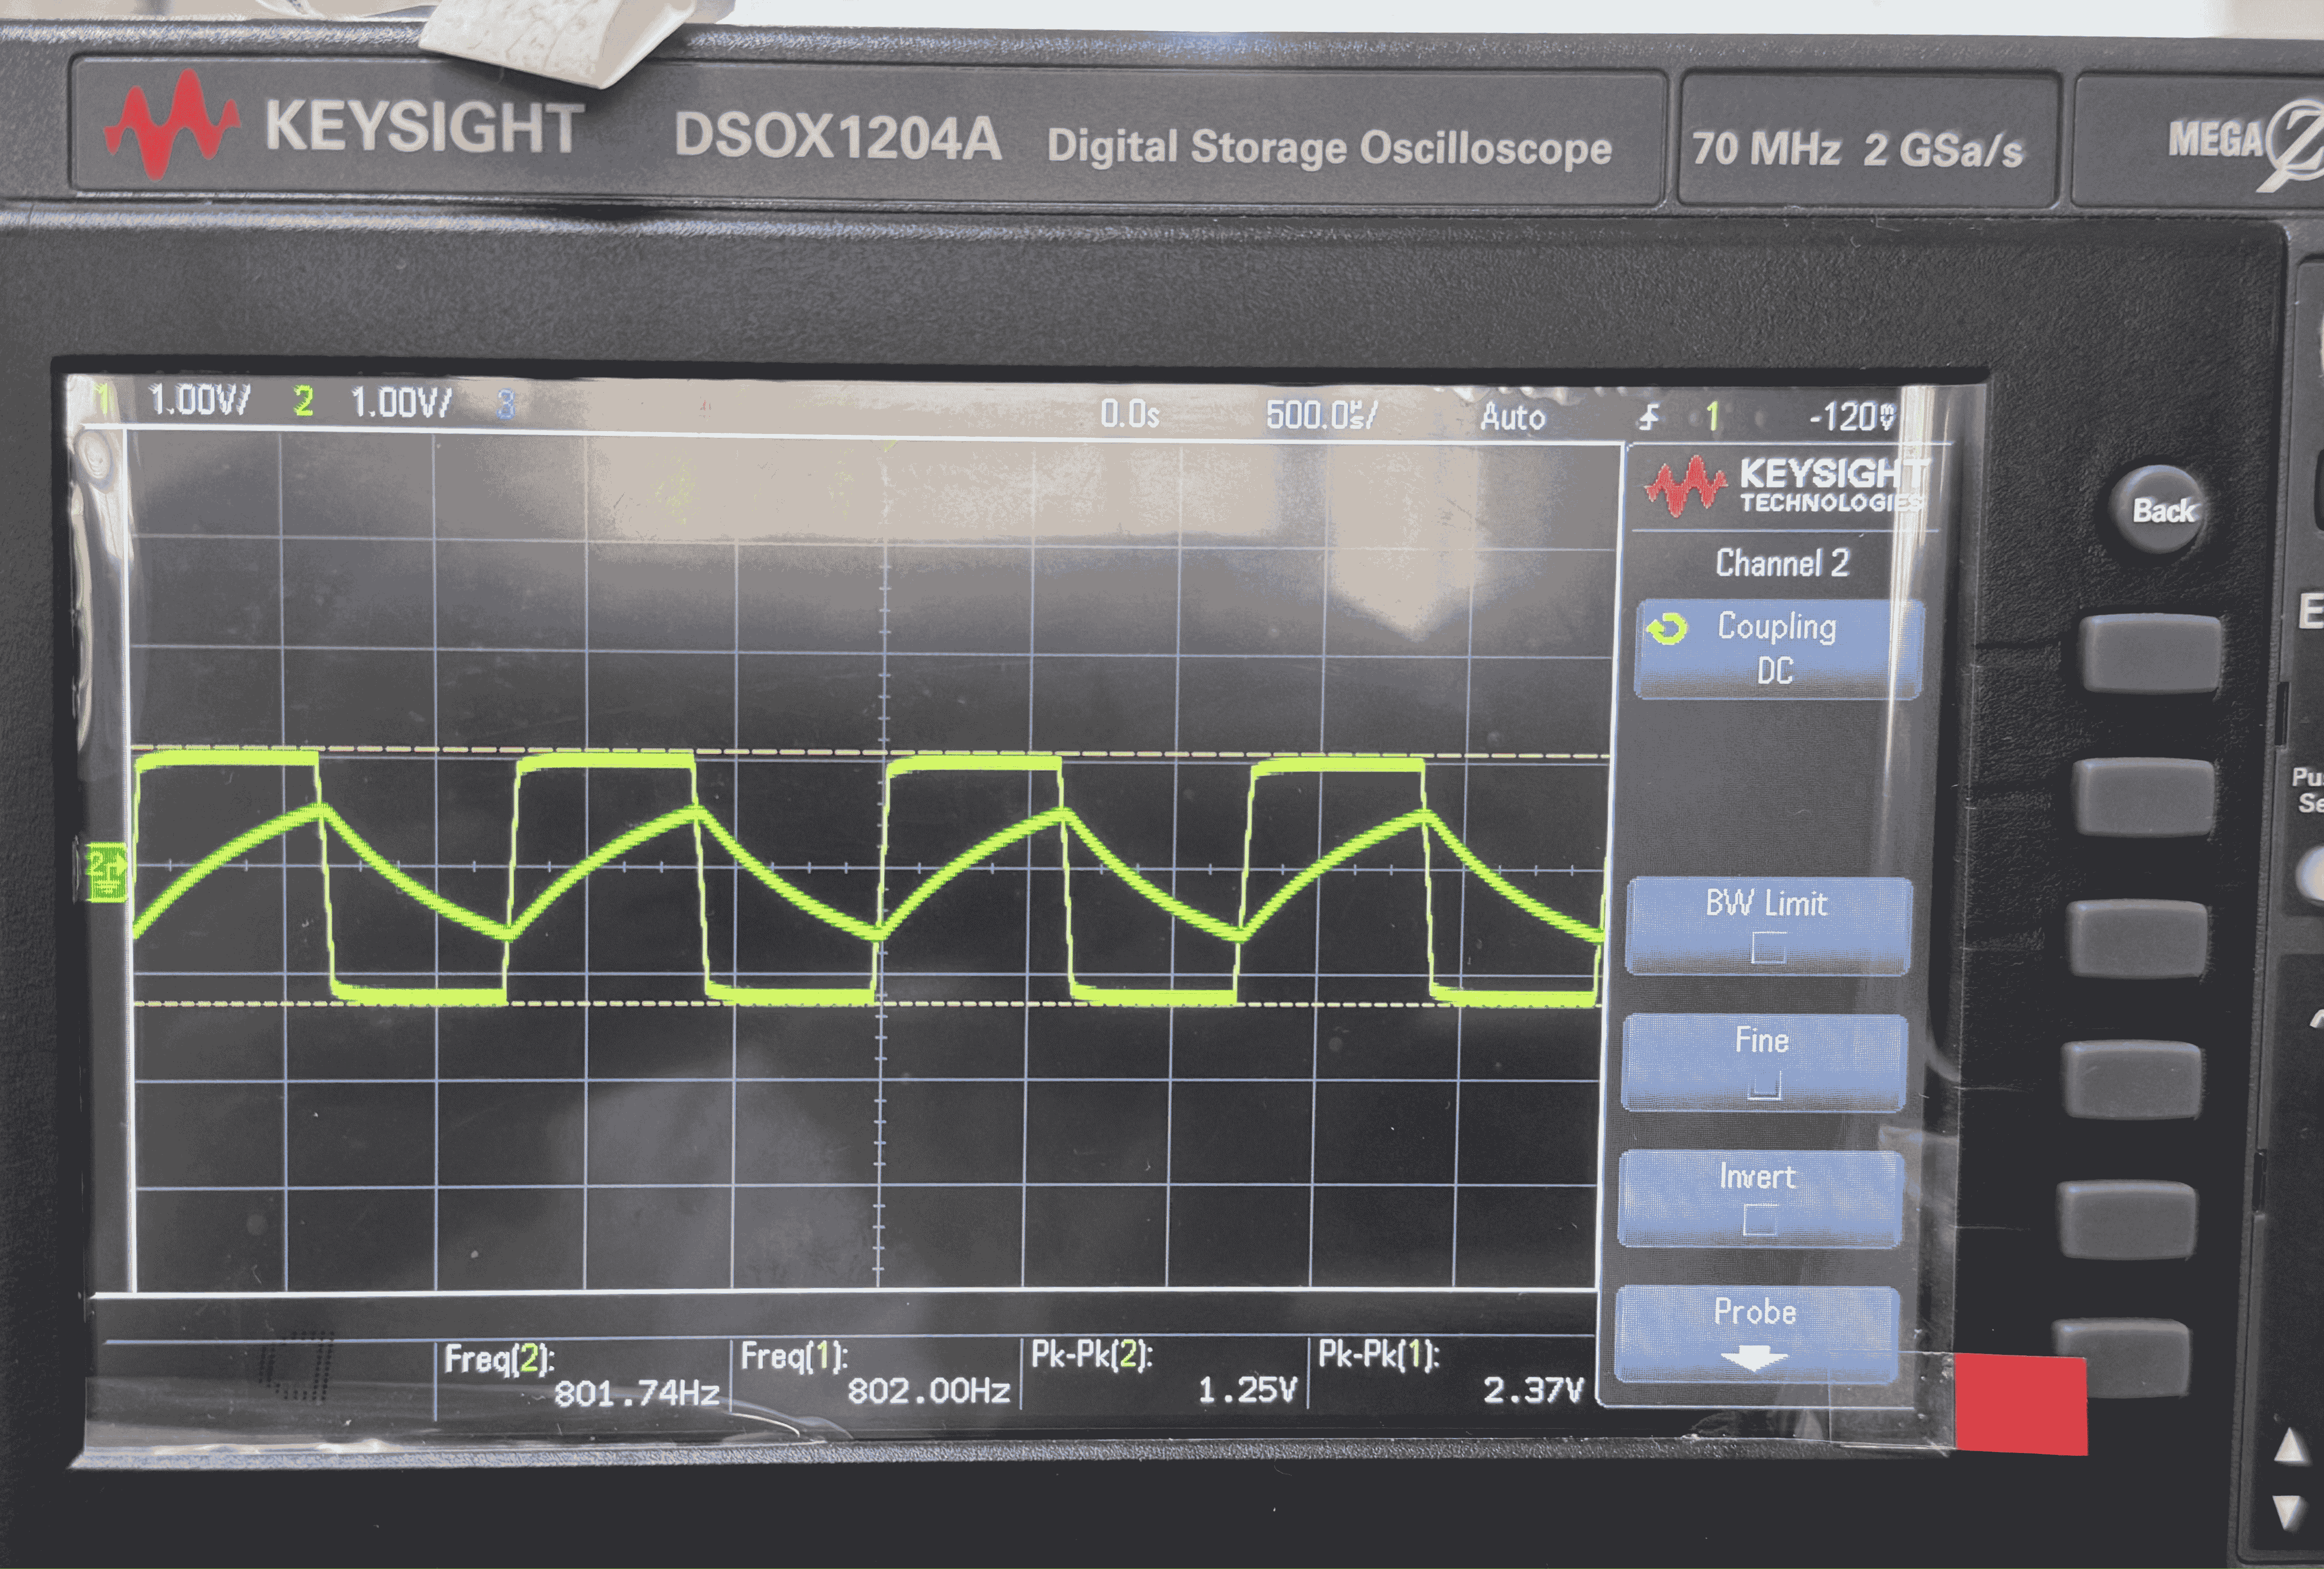
\includegraphics[width=0.95\linewidth]{Experiment_15/Images/5k5k.png}
        \caption{$R_4=5k\Omega,~R_5=5K\Omega$}
        \label{wave:15-5k5k}
    \end{subfigure}
    \begin{subfigure}{0.45\linewidth}
        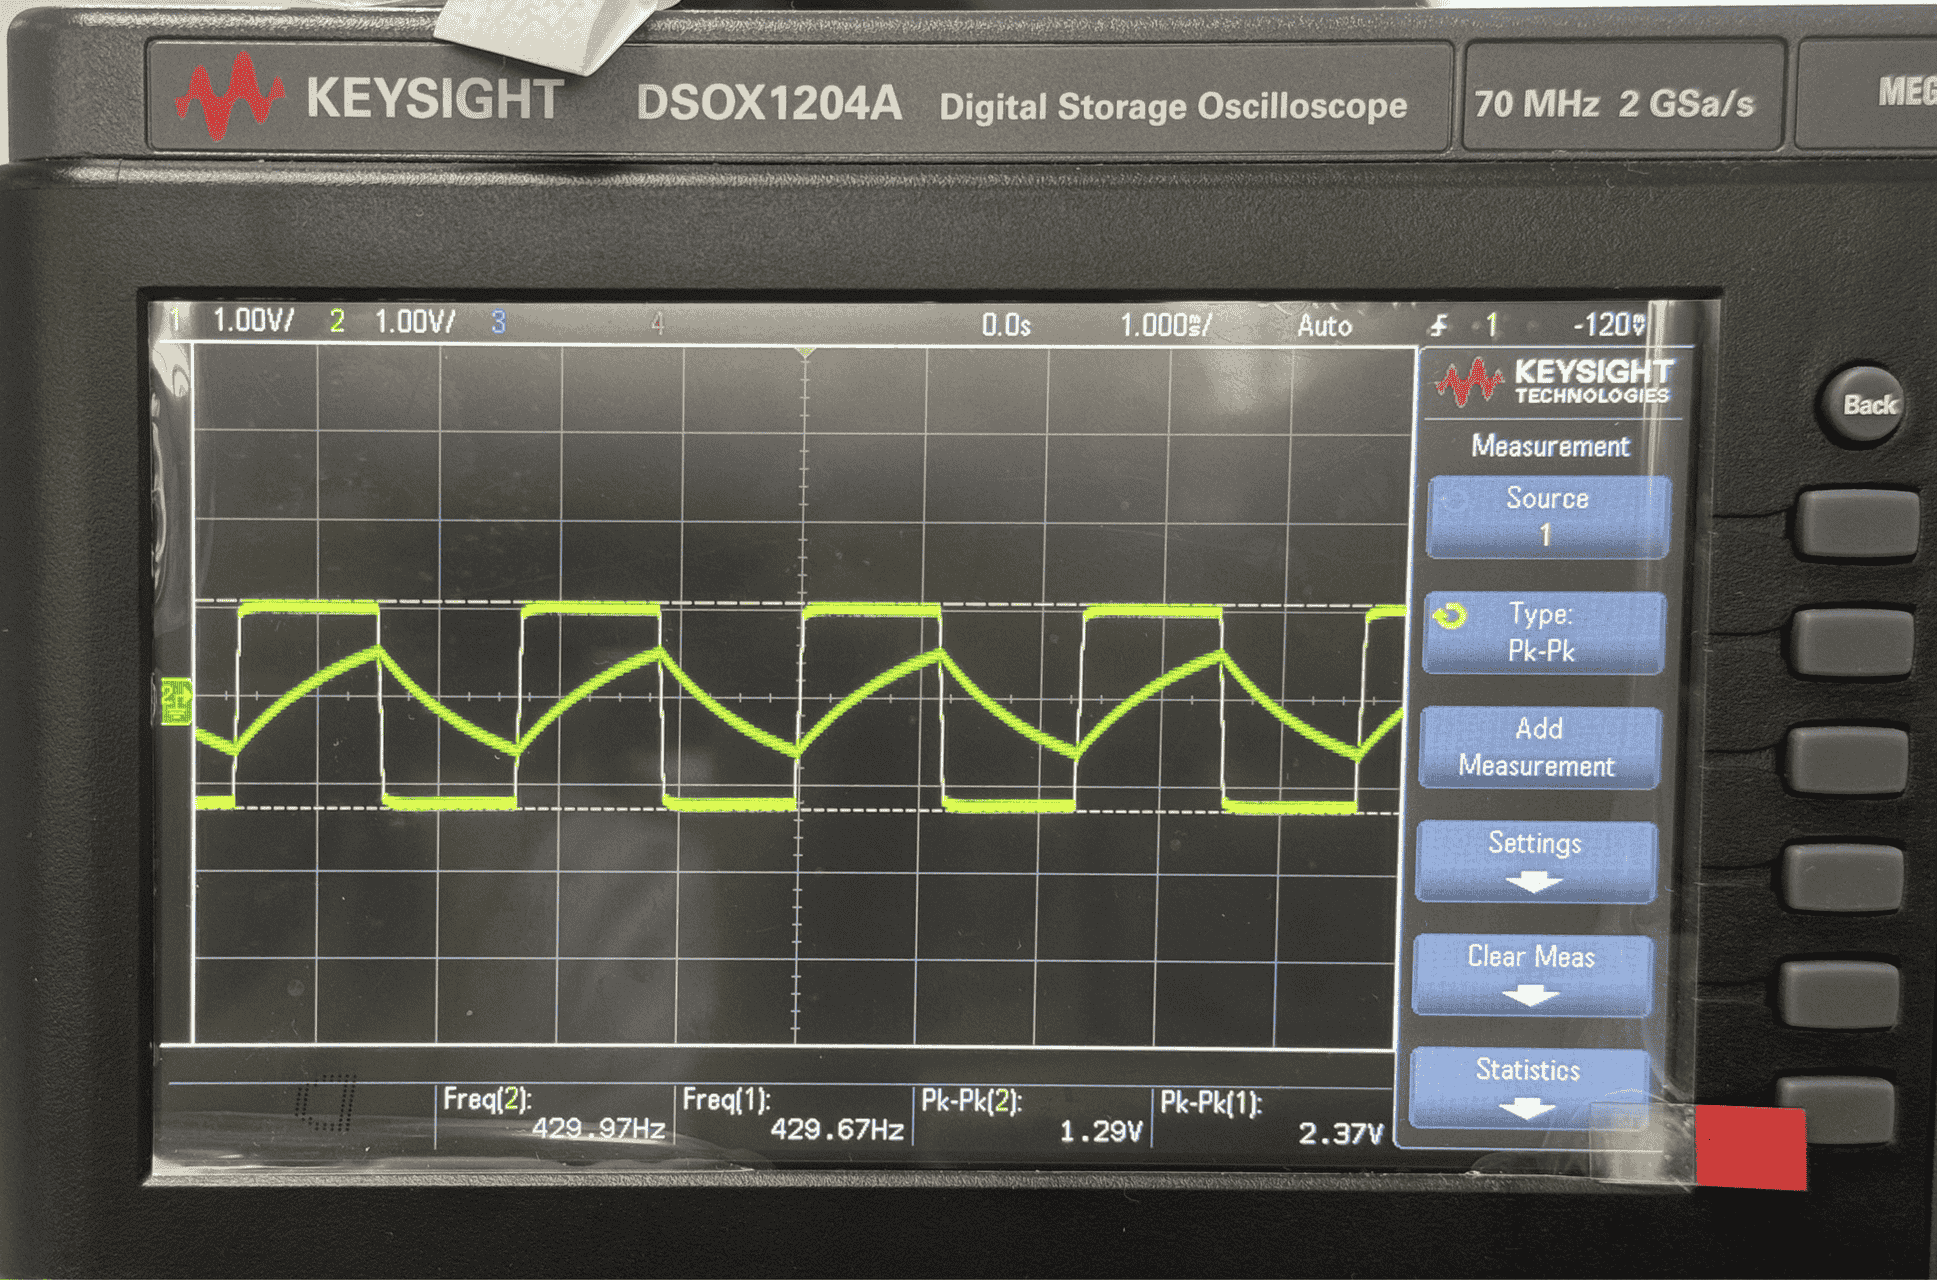
\includegraphics[width=0.95\linewidth]{Experiment_15/Images/10k10k.png}
        \caption{$R_4=10k\Omega,~R_5=10K\Omega$}
        \label{wave:15-10k10k}
    \end{subfigure}

    \begin{subfigure}{0.45\linewidth}
        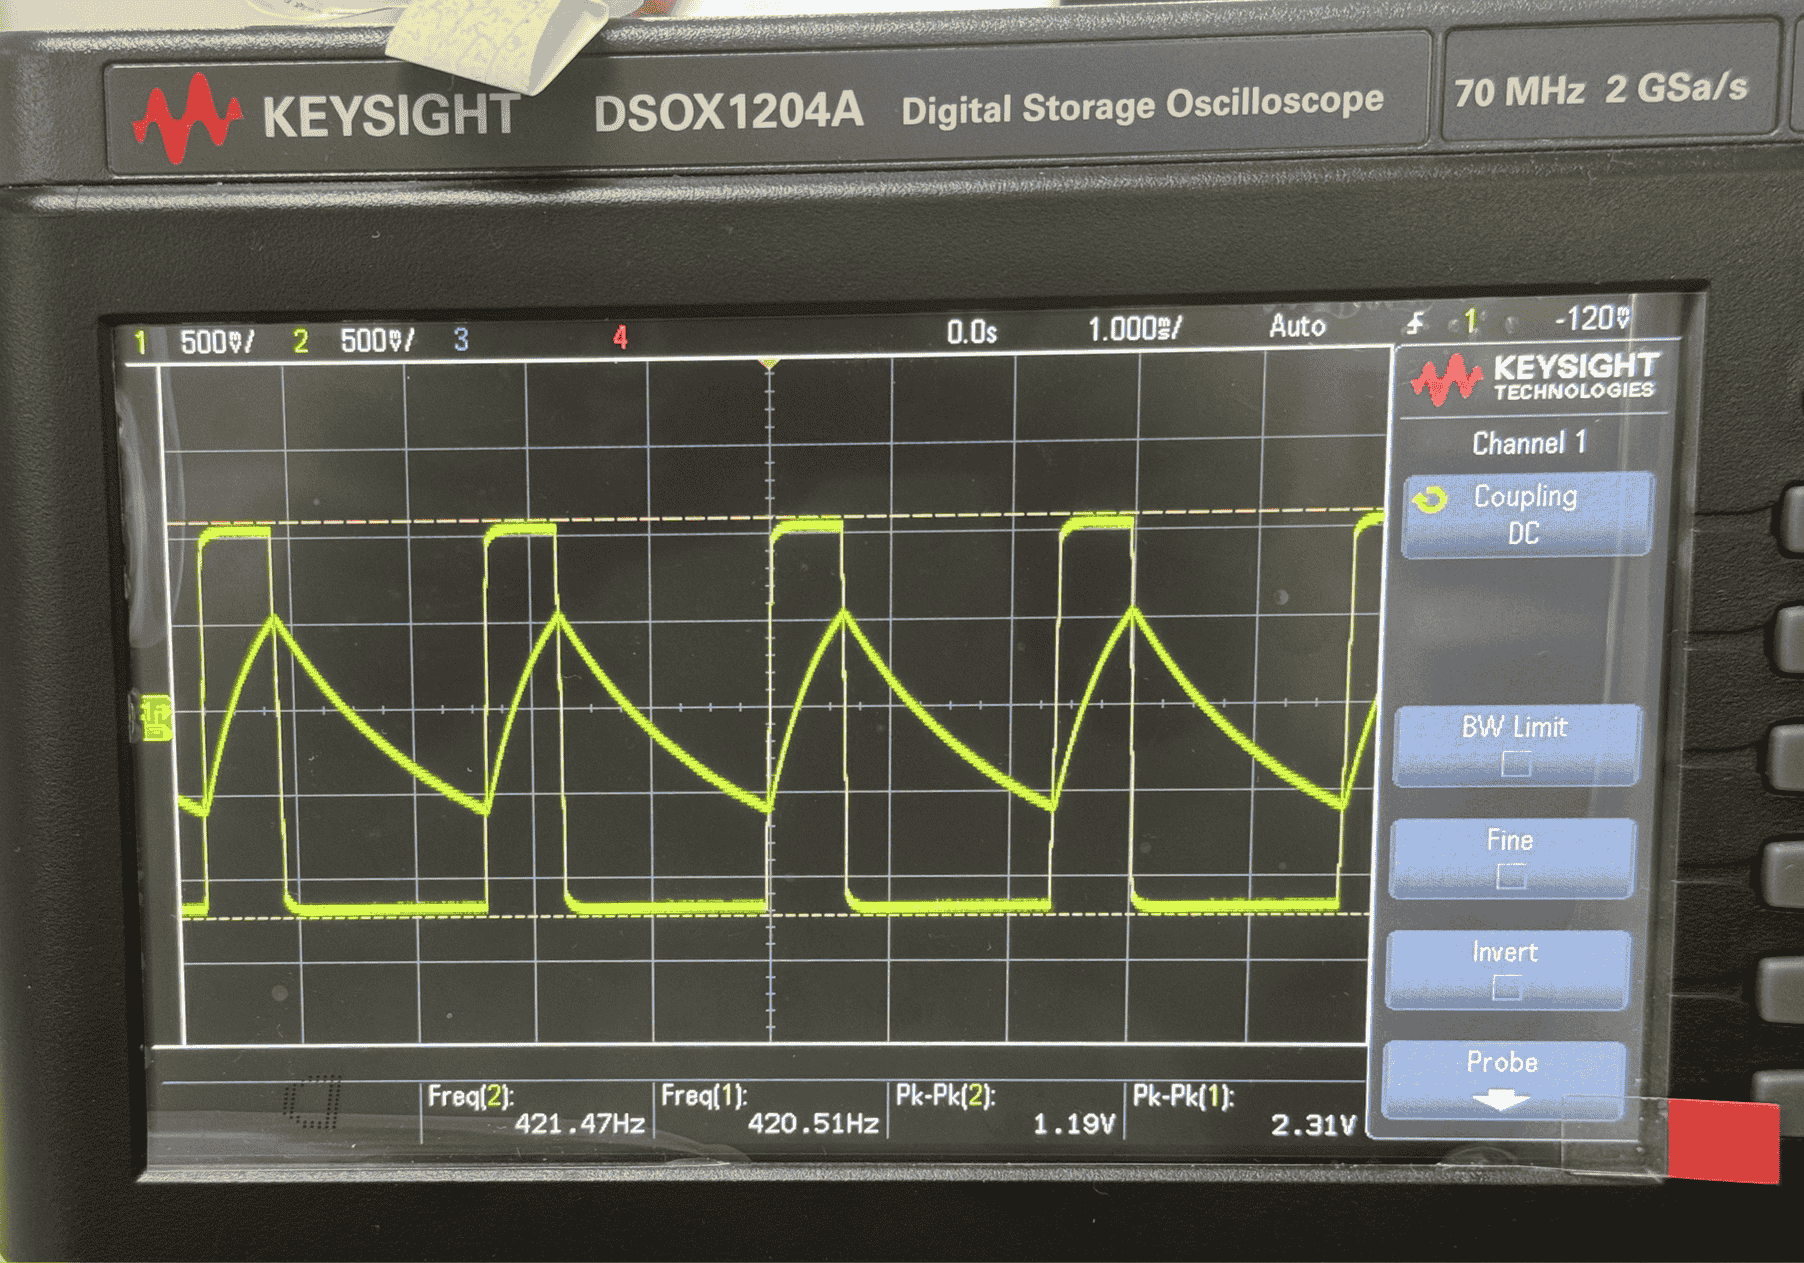
\includegraphics[width=0.95\linewidth]{Experiment_15/Images/5k15k.png}
        \caption{$R_4=5k\Omega,~R_5=15K\Omega$}
        \label{wave:15-5k15k}
    \end{subfigure}
    \begin{subfigure}{0.45\linewidth}
        
\includegraphics[width=0.95\linewidth]{Header/Empty.png}
    \end{subfigure}
    \vfill

    \caption{Observed Waveform of $R_4=R_5=10K\Omega$}
    \caption{Output signal and input signal waveform with different resistors}
\end{figure}


\FloatBarrier
The time required for the capacitor to charge and discharge is influenced by the resistors $R_4$ and $R_5$, respectively.\par
An increase in the resistance of the resistor governing the capacitor's behavior results in a longer period for the capacitor's voltage to change.\par
Conversely, a decrease in resistance reduces this period, as evidenced by the increase in the measured frequency ($f \propto \frac{1}{T}$) observed on the oscilloscope screen, as illustrated in Figure\ref{wave:15-10k10k} and Figure\ref{wave:15-5k5k}.
Therefore, when the resistance of two resistors ($R_4$ \& $R_5$) is different, it will result in an asymmetry duration of high signal and low signal states.

\subsection{Experiment Conclusion}
    \subsubsection{Conclusion}
        The square-wave generator circuit is a simple and effective way to generate a square wave signal. The frequency and duty cycle of the output signal can be adjusted by changing the resistors $R_4$ and $R_5$.
        